\documentclass[12pt]{article}

\usepackage[T1]{fontenc}
\usepackage{lmodern}
\usepackage{titling}
\usepackage{graphicx}
\graphicspath{{./images/}}
\usepackage{subcaption}
\usepackage[none]{hyphenat}
\usepackage{mathtools}
\usepackage{hyperref}
\usepackage[shortlabels]{enumitem}
\usepackage{float}
\usepackage{microtype}
\usepackage{tikz}
\newcommand*\circled[1]{\tikz[baseline=(char.base)]{
		\node[shape=circle,draw,inner sep=0pt] (char) {#1};}}

\usepackage
[
a4paper,% other options: a3paper, a5paper, etc
left=2cm,
right=2cm,
top=4cm,
bottom=4cm,
% use vmargin=2cm to make vertical margins equal to 2cm.
% us  hmargin=3cm to make horizontal margins equal to 3cm.
% use margin=3cm to make all margins  equal to 3cm.
]
{geometry}
\setlength{\droptitle}{-10em}

\title{Coursework 2}
\author{Dobrik Georgiev \\ \small dgg30@cam.ac.uk}

\begin{document}

\maketitle
~\\
\textit{\circled{1.} Describe Mobile Sensing challenges and its applications.}

Challenges:
\begin{itemize}
    \item Sensors are not very accurate. They are general purpose sensors, not
        specialised, so they have higher level of error. In addition to that
        position of sensors could vary, we can have different sensors that an
        application may use on a device (i.e. as in the same app on a device
        which has sensor X and on another which has sensor Y).
    \item Resources are constrained -- the app will be:
        \begin{itemize}
            \item Sharing resources with many other apps -- it's running on
                a mobile device, not a dedicated, where there is an OS which
                would not dedicate the whole CPU/Memory to a single app.
            \item Running on a battery powered device -- sensing is resource
                expensive and drains battery. It also reduces device
                performance (I have had sensing apps ages ago that made my
                phone work slower.).
        \end{itemize}
    \item There are privacy concerns -- sensing could reveal private data about
        the life of the user (lifestyle, habits, current location, mood, etc.)
    \item Given all of the above the app still needs to provide accurate enough
        data, so that it is still useful -- needs to strike a balance between
        resource usage and accuracy.
\end{itemize}

Applications:
\begin{itemize}
    \item Monitoring human activity -- fitness, health (heart rate, etc), sports, etc
    \item Transport-mode detection -- contributes to identifying the needs of
        workers (travelling time, transportation choice, etc.) and supporting
        creating commuting services to meet the needs
    \item Emotion detection
    \item Context and Environment applications -- automated diary, etc.
    \item Fancy voice control -- e.g. Alexa/Siri and similar products
    \item and many, many, other ubiquitous applications that could fill a whole supervision slot if I started listing them$\dots$
\end{itemize}
\textit{\circled{2.} Describe how inference of activity can be done in mobile
phone sensing applications.}

Gathering (labelled) data: User actions such as speech, motion, Wi-Fi, GPS,
etc. and label data is gathered and a probabilistic ML model can be built. Each
of the different sensor measurements can be grouped into a single feature
vector and we can use something like SVM to perform classification/regression.
(Alternatively, we can have separate learners for each sensor and ensemble
these to infer the activity).

However, there are some issues:
\begin{itemize}
    \item Noisy sensors and complex world data often cause confusion to the
        classic ML algorithms. Deep Learning and Deep Neural Networks could be
        helpful here, as they are more robust. However, their integration into
        mobiles and wearables is complicated because of resource constraints.
        There are attempts to overcome this both in terms of hardware (e.g. my
        phone has a dedicated Neural Processing Unit) and in terms of software
        (e.g. the paper by S. Bhattacharya and N.D. Lane).
    \item Gathering labelled data is also somewhat not straightforward, though
        more and more datasets are released for free use every day.
    \item There are always concerns about privacy of the user and similar
        law-related things.
\end{itemize}
\textit{\circled{3.} Describe what are the main challenges in running machine
learning algorithms entirely on mobile devices.}

Building up on what I said in the previous question, I could add the following: \begin{itemize}
    \item Running ML/DeepL consumes a lot of power and drains battery -- it might
        be beneficial to \emph{sometimes} upload the sensed data and do the
        inference on the cloud. However, some other times, uploading itself may
        use a lot of resources so, it could be better to keep doing the
        computation on the device.
    \item Training models -- at this moment mobile devices are not very capable
        of training a Neural Network from scratch, because they are limited in
        computational power (training the algorithm takes CPU power) and in
        memory (the more diverse the dataset, the better the results, the
        larger the memory needed to store it). E.g. imagine to have to train
        a model on Imagenet, but on a smartphone.
\end{itemize}
\textit{\circled{4.} Describe Context Sensing Sharing.}

The idea is that continuous sensing takes a lot of battery, whereas duty
cycling may not give a good estimate of user actions. Therefore each time some
app uses some sensor X, the OS caches it and when at a later time when another
app uses the same sensor X the cache value is returned (assuming it's
reasonably close in time, e.g. you can't use cached value of accellerometer
5 hours later).

\emph{Side Note: I understand that CrossApp Context Sharing $\neq$ Shared
Context Sensing.}
\\
\\
\textit{\circled{5.} Describe the architecture and components of ACE.}

\begin{figure}[H]
    \centering
    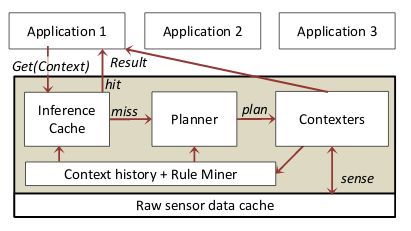
\includegraphics[width=250pt]{ACE_Architecture.png}
\end{figure}
\begin{enumerate}[1.]
    \item Contexters -- collection of modules, each of which determines the
        current value of a context attribute (e.g.,IsWalking) by acquiring data
        from necessary sensors and by using the necessary inference algorithm.
        An application can extend the contexters. Note that ACE treats
        contexters as black boxes; the only two pieces of information
        a contexter needs to expose to ACE are the name of the attribute that
        it determines (\textbf{IsWalking}, \textbf{IsDriving}, $\dots$), and
        its energy cost.

    \item Raw sensor data cache -- classic cache to share recent measurements.

    \item Rule miner -- The rule miner component of ACE maintains a history of
        timestamped tuples (e.g., \textbf{AtHome=True}), sensed for various
        applications. It then incrementally derives rules regarding
        relationships among various context attributes. It uses the Apriori
        algorithm for rule mining, which can efficiently discover association
        rules from databases containing transactions. Since in ACE various
        contexters may be invoked for different applications
        asynchronously\footnote{To derive $A \Rightarrow B$, we need both A and
        B to appear together in the same transaction.}, we need to batch them
        as a single transaction of co-occurring tuples. This could be done
        by:
        \begin{itemize}
            \item Using a fixed time window -- choosing the right window size is tricky
            \item Using a dynamic window size -- a default window size is used,
                but it's trimmed if the value of any context attribute changes,
                in order to avoid conflicting tuples in one window. Windows
                having a single tuple are also ignored.
        \end{itemize}

        The rule miner also deals with inaccuracies (by regularly
        crossvalidating with ground truth) and also removes redundant rules by
        compacting them, in order to reduce inference overhead.

    \item Inference cache -- Used for intelligent context caching, e.g. if an
        app asks for the value of \textbf{Driving} but we have recently cached
        that \textbf{AtHome=True} then we can return \textbf{Driving=False}.
        We can reuse values not just for an exact lookup, but for semantically
        related lookup.

        In terms of API it has a Get/Put interfaces, and whenever a Get(X) is
        in the cache, returns it. Get(X) also returns value of X if X is not 
        directly in the cache but also, if it can be inferred by using context rules
        and cached values of other attributes

        The inference cache uses expression trees (trees which represent boolean expressions)
        to efficiently exploit the rules. The expression tree is built in a way that can
        handle transitive relationships between the rules. One expression tree is 
        maintained for each tuple, i.e. for \textbf{Driving=True} and \textbf{Driving=False}
        we have 2 trees. On a Get request of \textbf{X} both trees for it are evaluated and
        a result is returned.

        As the expression trees could become really large and we want to reduce the
        memory overhead of using trees for the expressions, the trees are compacted 
        using standard boolean algebra:
        \begin{itemize}
            \item Alternating AND-OR level.
            \item Absorption
            \item Collapse
        \end{itemize}

    \item Sensing planner -- On a cache miss this finds the sequence of attributes to
        speculatively sense in order to determine the value in the cheapest way. The 
        sensing planner can build a plan which orders the attributes to check based
        on their cost to sense and probability to be True (or False). E.g if we 
        want to infer if the user is in a meeting, we can go for the `classical' way
        or we can do a sequence of steps, through which we can infer the attribute in
        a cheaper way. Note that in the worst case, the path taken could be more costly
        than directly sensing the needed attributes, but ACE algorithms for speculative
        sensing minimize that probability.
        \begin{figure}[H]
            \centering
            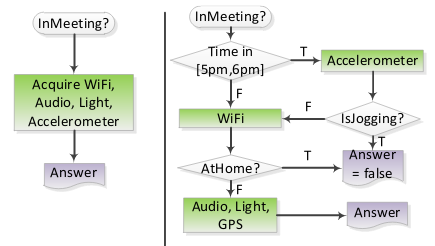
\includegraphics[width=250pt]{conditional_plan.png}
        \end{figure}
\end{enumerate}
\textit{\circled{6.} Illustrate the advantages of a dynamic offloading of
computation model like in MAUI and the trade offs to be considered..}

Advantages:
\begin{itemize}
    \item MAUI's primary goal is to reduce the energy consumption of mobile
        applications. 
    \item In addition to saving energy, MAUI can also
        improve the performance of mobile applications.
    \item Allows
        developers to build applications that cannot currently be supported on
        mobile devices because of their resource requirements.
\end{itemize}
  
The trade offs to be considered are:
\begin{itemize}
    \item \emph{How much does MAUI reduce energy consumption of mobile
        applications?} --- According to the MAUI paper, when the server is nearby
        the energy savings can reach one order of magnitude (10x). As the
        latency to the server increases, MAUI saves less energy. In fact, the
        energy consumed when offloading code over 3G is 2.5x higher than
        offloading code to a nearby server.
    \item \emph{How Much Does MAUI Improve the Performance of Mobile
        Applications?} --- For nearby servers and low latency, results showed
        that offloading improves performance. However, for a RRT higher than 25
        ms, some apps' performance can be hurt (as the chess game experiments in
        the paper). The worst case performance is when offloading over 3G -- the
        method for selecting piece in the chess game incurred 77\% performance overhead,
        whereas the videogame incurred 54\%.
    \item \emph{Can  MAUI  Run  Resource intensive Applications?} --- Results showed
        that MAUI can bypass smarthone's limits on an application's memory footprint
        (e.g. there is a result, where peak memory consumption was 110MB whereas the
        phone had 32-48MB RAM).
    \item \emph{What is the Overhead of MAUI's Optimizer?\footnote{Recall that
        MAUI has to profile the usage of the app and solve a 0-1 integer linear
        problem, in order to decide where it should execute the function.}} ---
        Experiments showed that the solver takes 18ms on average to solve for a
        chess game and 46ms for the video game.
    \item \emph{Is MAUI Effective at Identifying Code Offload Based on a Global
        View of a Program?} --- Certain programs, e.g. face recognition, can
        have a functions that on their own execute using less resource/faster,
        but combined are better to be offloaded Compared to a naive solver,
        which views all methods locally, MAUI performed better.
    \item \emph{How Effective are Incremental Deltas at Reducing MAUI's Data
        Transfer Overhead?\footnote{Deltas, i.e. transferring just state
        changes instead of entire state.}} --- When experimenting with
        the videogame, MAUI reduced the amount of offloaded information
        by a factor of 2 (23KB to 12KB).
\end{itemize}
\textit{\circled{7.} The Bat system is a ToF (Tome of Flight) system where the
tag acts as a transmitter.}
\begin{enumerate}[i)]
    \item \textit{Explain how sync is obtained.}

        (A \textit{sync}? I'm sorry for not being able to `read between the lines' but can you clarify what is meant by sync.)

        A base station periodically transmits a radio message containing
        a single identifier, causing the corresponding Bat to emit a short
        unencoded pulse of ultrasound. Simultaneously, the ultrasound receivers
        in the rooms covered by the base station are reset via the wired
        network. Receivers monitor the incoming ultrasound and record the time
        of arrival of any signal from the Bat. Using the speed of sound in air
        (which can be estimated from the ambient temperature), the times of
        flight of the ultrasound pulse from the Bat to receivers can be
        converted into corresponding Bat-receiver distances. The position of
        the object attached to the Bat can be then deduced by multilateration.

        After a distance-measuring pulse has been emitted, the base station
        waits for reverberations of the pulse to die out before triggering
        another Bat, ensuring that receivers can ascribe incoming ultrasonic
        signals to the correct Bat. This process divides time into timeslots,
        each of which can be used to locate a single Bat. (Roughly 20ms per
        slot.)
    \item \textit{Describe how to invert the system so that the tag is a receiver.}

        That's a tricky one -- when the Bat is a receiver you cannot just transmit from
        all transmitters, assuming transmitters are on the ceiling and that they use one and
        the same frequency. We need to do some `hacks' in order to circumvent the fact that
        the Bat is a receiver:
        \begin{itemize}
            \item Let transmitters have a unique code (e.g. like a barcode of
                flickering sound or different frequency for each transmitter).
            \item Transmitters will transmit in time multiplexed manner -- one
                transmitter per slot, there is always someone transmitting.
                Alternatively, they can transmit in a frequency multiplexed
                manner -- one transmitter per frequency band, all transmitters
                transmit at once at the same time and then go silent for a period
                of $\delta t$.
            \item If we choose time-multiplexing, the Bat will need to be
                sensing all the time and remember which transmitters it heard
                (e.g. sensing 1, 5, and 6 one after the other). If we go for
                frequency multiplexing, the Bat will need to be sensing all the
                time for at least the synchronisation period when it enters the
                system. After that, it can infer and keep a schedule which is
                the same as the transmitters'. Alternatively, the schedule
                could be given to the bat by the base station.
            \item The Bat will need to have a mapping between the code of the
                transmitter and it's location and perform the relative
                multilateration computation itself. (I assume offloading of the
                data would be as expensive as the computation itself.)
            \item The Bat reports its location to the base station, in the case
                where we want the location to be open to other people (i.e.
                seeing when sb is in its office).
        \end{itemize}
        These should be enough for localising the Bat.
    \item \textit{Discuss the advantages and disadvantages of this alternative approach.}

        Disadvantages: Bat having to `listen' (in FDM less frequently, but
        still...); Bat having to have a mapping and having to compute its own
        location (or do offloading of data). All of these 1) incur overhead, 2)
        waste Bat's battery life a lot more than the classic approach.

        Advantages: Assuming the Bat is more like today's smartphones and the disadvantages
        are acceptable, we can handle as many Bats as we want, since the system is `decentralised'
        (sort of) and the base station could handle many more devices.
\end{enumerate}
\textit{\circled{8.} Imagine that you are tasked with designing an iPhone-like
device that must be able to position itself at all times (indoors and out).
Discuss the solutions you could use and the accuracies you might expect indoors
and out.}
\\
Outdoors:

Most likely, I would go for using GPS/GNSS.  I would expect accuracy of around
3-4 meters (varies between exact solution used). Other tricks could give better
accuracies, e.g. Carrier Phase positioning gives ~20cm, but you need an
accurate initial location and more time. Given it's an iPhone-like device, the
user might be likely to want to use it immediately and keep walking while being
guided with it, not to wait 15 minutes for an initial location.

Alternatives such as cellular localization may be an option, when GPS is not
really suitable (e.g. you are in Manhattan, skyscrapers, you get it), but the
accuracy from such methods is lower.
\\
\\
Indoors:

There are many alternatives. A first classic alternative would be to use BLE
beacons.  The device can detect the signal from the beacons and can calculate
roughly the distance to the beacons to build an estimate for the location.
Companies like Bloomberg have such things deployed for indoors localization.
Accuracy can vary, but can be as good as ~1.5m. (That's what I'd probably go for)

Another alternative would be using Wi-Fi to determine location -- using some
sort of Nearest Neighbour in Signal Space. This needs identifying signal at
prespecified locations offline and then the mobile device can scan the Wi-Fi,
build an observation vector and find the `nearest' vector of the measurements.
(Or you could use regression to create continuous probabilistic map for each
base station.) Unfortunately, this approach suffers from several problems --
poor geometry of APs, body shadowing, changing environments, scanning costs,
room ambiguity (two rooms can have the same/similar measurements), etc.

Yet another WiFi solution could be FTM (Fine Timing Measurement), which assumes
that phone and AP can be unsynced, but they have to have a good quality timing
(i.e. fine timing). The localisation is done computing ToFs from different 
stations and use multilateration.

Optical solutions can also be an option, but it is going to be way too
complicated to attach photosensors on the device (as in the Valve's Lighthouse
product) and have lighthouses at different places on top of that.

There are other possible solutions as well, e.g. Phased Arrays, but I don't
think they would be any better (needs evenly spaced antennas and
reflection+mulitpath is a problem).

(I can't really find information what accuracies do the last solutions produce
-- can we just mention them on the supervision.)
\\
\\
\textit{\circled{9.} Describe the principles underlying the Kalman Filter. Why
is it so commonly used? What does the H matrix in the Kalman Filter
represent?} 

At the start we have some Gaussian PDF estimating the initial position. As we
move, we use the motion model to update the PDF and \textit{predict} where we
are. Motion model can vary between different examples, but should be possible
to model it using linear algebra, e.g. $x_t = F_tx_{t-\delta t} + w_t$, where
$F_t$ is the matrix describing the motion model (can vary), xs are states in
time and $w_t$ is a noise term (can also vary).  The uncertainty (which is
modelled by a covariance matrix) needs also to be updated: $P_t
= F_tP_{t-\delta t}F^T_t+Q_t$ (Q is a noise term).

Then we \textit{predict} what would the measurements would be too, based on our belief about the
state.
\begin{gather*}
    \mu_{expected}=H_tx_t
    \\
    \Sigma_{expected}=H_tP_tH^T_t
\end{gather*}
The H matrix models how our state relates to the measurements (this could be as
simple as (1 0) as in the lecture notes or could be complex if our measurment
has different units/scale)

Then, given our measurements producing another $\mu_t$ and $\Sigma_t$
(measurements have Gaussian PDF too) we will combine them by simply multiplying
the two Gaussians together, which will produce another Gaussian, giving the
probability both the expected and real measurements are true and
\textit{update} our belief for the state based on these
probabilities\footnote{I'm referring to equations 14 to 19 in
\url{http://www.bzarg.com/p/how-a-kalman-filter-works-in-pictures/}}.

The reasons KFs are commonly used is (quoting Dr R. K. Harle): "Because why
not?". Everything boils down to linear algebra and matrix multiplications, for
which a CPU is optimised for, i.e. they are cheap to compute. Moreover KF and
EKF are algorithms and not heuristics, so as long as some preconditions, such
as our system is a linear system with Gaussian noise, are met, KFs guarantee
optimality.
\\
\textit{\circled{10.} Discuss the extent to which you can speed up a particle filter using parallel processing.}

Clearly you can parallelise the UPDATE and CORRECT step, as the same operations
are applied to each particle (in Flynn's taxonomy, it is SIMD). What is
difficult to parallelise is the resampling step, where a CDF of the particles'
probabilities has to be formed and this is not (easily) parallelisable. A quick
search online led me to
\url{https://docs.nvidia.com/cuda/cuda-samples/index.html#cuda-parallel-prefix-sum--scan-},
which \textit{should} be an implementation of prefix sum, which should be
enough for creating the CDF. Sampling can also be done in parallel. However,
this is a solution for GPUs, not embedded CPUs as those on your phone, so it 
may not be very suitable solution.
\end{document}
